%
% teil2.tex -- Beispiel-File für teil2 
%
% (c) 2020 Prof Dr Andreas Müller, Hochschule Rapperswil
%
% !TEX root = ../../buch.tex
% !TEX encoding = UTF-8
%
\section{Umsetzung - Programm 
\label{wavelets:section:teil2}}
\rhead{Teil 2}

\subsection{Einleitung
\label{wavelets:subsection:Einleitung}}
Die folgende Passage dient der Herleitung des CWT-Codes. Dabei liegt der Fokus mehr auf den Hürden und Erkenntnissen und weniger auf den einzelnen Code-Zeilen. Es handelt sich nicht um eine wie man es am besten macht Anleitung, vielmehr wird der Weg hin zu einem lauffähigen CWT-Code beschrieben.
Das verwendete Mutterwavelet ist ein Morlet Wavlet \[\psi(a,b)=Ke^{-j2\pi f_0\left(\frac{t-b}{a}\right)-\frac{\left(\frac{t-b}{a}\right)^2}{2}},\] dass sich, wenn man es auf die reale Ebene projiziert aus folgenden zwei Komponenten zusammensetzt:
\begin{itemize}
	\item $e^{-j2\pi f_0\left(\frac{t-b}{a}\right)}$ Cosinus mit der Frequenz $f_0$ (Grundfrequenz des Mutterwavelets), dem Skalierungsfaktor der Frequenz über die Laufvariable a sowie der zeitlichen Verschiebung b.
	\item $e^{-\frac{\left(\frac{t-b}{a}\right)^2}{2}}$	Gauss Gewichtungsfenster an der Stelle der Verschiebung b mit der Skalierung $\frac{1}{2a^2}$.
\end{itemize}

Die Abbildung unten zeigt wie das Morlet-Wavelet aus den beiden Anteilen erzeugt wird (Abbildung \ref{wavelet:fig:MorletWavelet}).

\begin{figure}
	\centering
	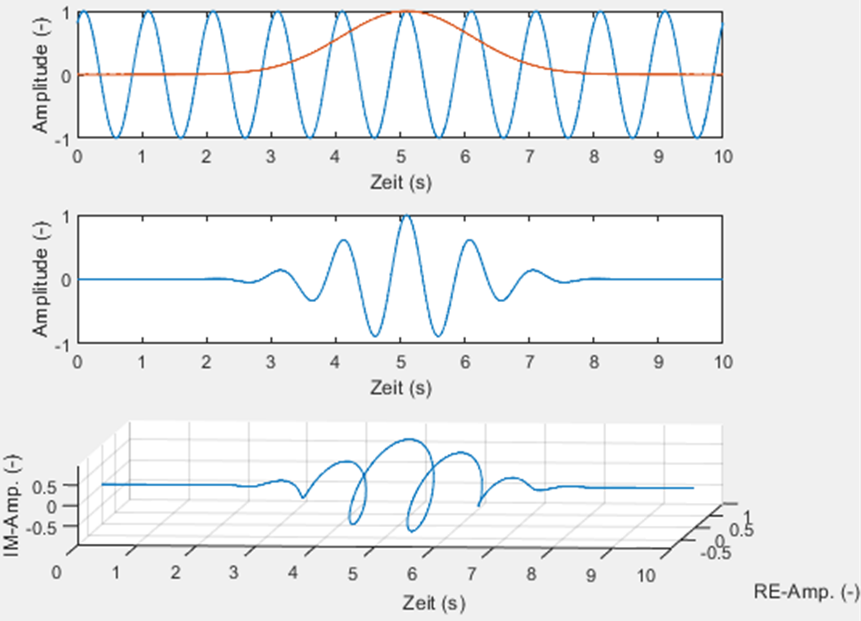
\includegraphics[width=0.3\textwidth]{papers/wavelets/images/7_MorletWavelet.png}
	\caption{Graphischer Nachvollzug zur Erzeugung des Morlet Wavelet, in blau der Cosinus und in orange das Gauss Gewichtungsfenster. Darunter die Ansicht des auf die reale Ebene projizierten sowie des komplexen Wavelets.}
	\label{wavelet:fig:MorletWavelet}
\end{figure}

\subsection{Phasenverschiebungskorrektur
	\label{wavelets:subsection:Phasenverschiebung}}
Die erste Hürde war die Phasenverschiebung in der Erzeugung des Morlet Wavelt. Wenn bloss die Amplitude von Interesse ist, spielt die exakte Phase durch die komplexe Verrechnung keine Rolle. Jedoch wie sich in der Untersuchung der Eigenschaften des Wavelets noch zeigen wird, nimmt der Phasenverlauf eine spannende Funktion in der zeitlichen Auswertung ein. Deshalb war eine korrekte Phasenverschiebung zielgemäss. Die Gegenüberstellung zeigt wie sich eine falsche Phasenverschiebung auf das Morlet-Wavelet auswirkt (das Wavelet in Abbildung \ref{wavelet:fig:PhaseShiftFailVsCor} wird in der Projektion auf die Reale Ebene unsymmetrisch).

\begin{figure}
	\centering
	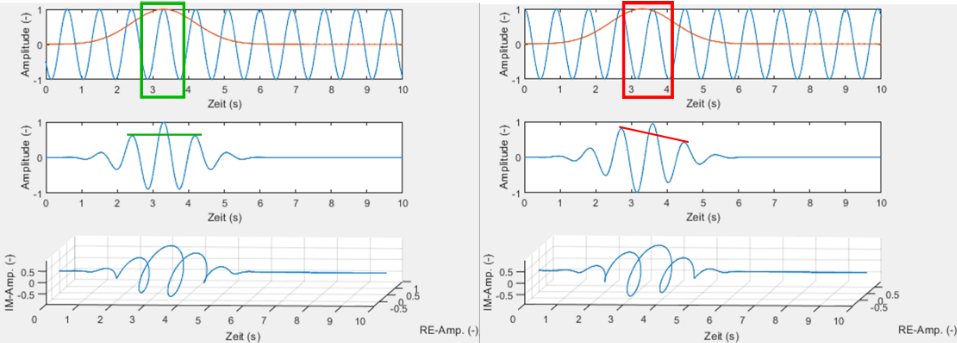
\includegraphics[width=0.7\textwidth]{papers/wavelets/images/9_PhaseShiftFailVsCor.png}
	\caption{Einfluss der Phasenverschiebung auf das Wavelet betrachtet an der Projektion auf die reale Ebene}
	\label{wavelet:fig:PhaseShiftFailVsCor}
\end{figure}

Der Weg zur Implementierung der korrekten Phasenverschiebung war ein kleiner drei Satz (Abbildung \ref{wavelet:fig:PhaseCalc}).

\begin{figure}
	\centering
	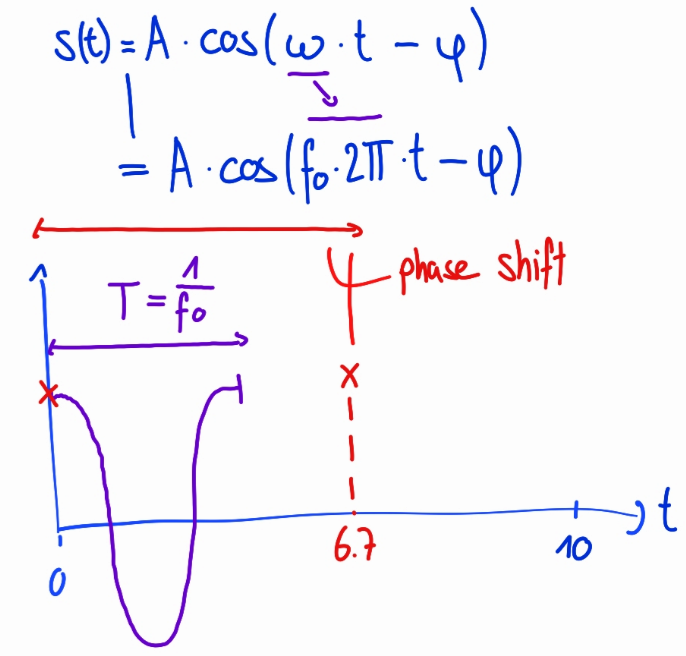
\includegraphics[width=0.25\textwidth]{papers/wavelets/images/10-1_PhaseCalc1.png}
	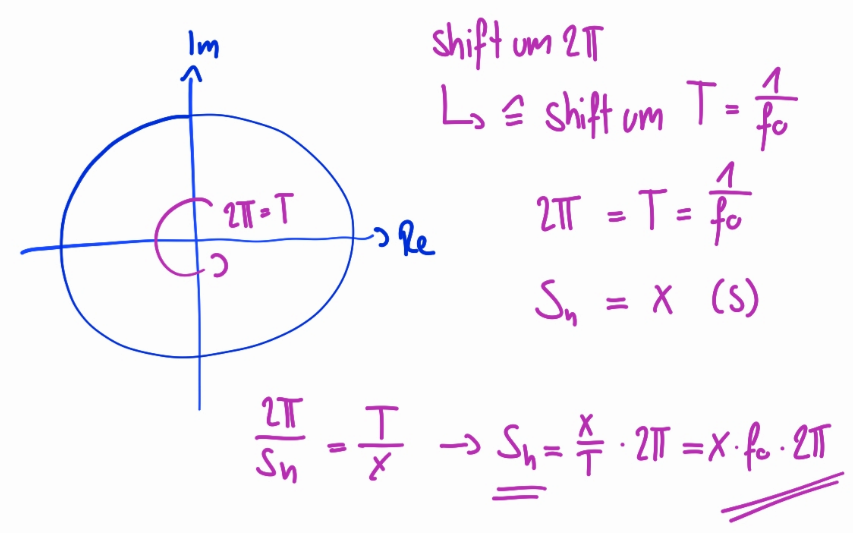
\includegraphics[width=0.3\textwidth]{papers/wavelets/images/10-2_PhaseCalc2.png}
	\caption{Dreisatz zur Berechnung der korrekten Phasenverschiebung.}
	\label{wavelet:fig:PhaseCalc}
\end{figure}

In der Abbildung \ref{wavelet:fig:PhaseCalc} links zeigt sich die Wunschvorstellung, anhand einer fiktiven zeitlichen Verschiebung von 6.7s. Dabei stellt sich die Frage, um wie viel muss die Phase des Cosinus verschoben werden, damit dieser exakt nach 6.7s wieder bei 1 startet. Damit das Morlet Wavelet auf die reale Ebene abgebildet symmetrisch erzeugt wird.
Mit Hilfe des Einheitskreises kann dieses Problem relativ einfach nachvollzogen und gelöst werden (Abbildung \ref{wavelet:fig:PhaseCalc}). 
Eine Umdrehung entspricht gerade $2\pi$ und das ist bei der Grundfrequenz von $f_0$ eine Periodenlänge von $T=1/f_0$. Also muss meine Phasenverschiebung für ein bestimmtes b (zeitliche Verschiebung des Wavelets) gerade $S_h=b\cdot f_0\cdot 2\pi$ entsprechen ($S_h$ steht hierbei für Shift, also die zeitliche Verschiebung). Für die Umsetzung in der Programmierung spielt natürlich die gegebene Frequenz, welche die Skalierung von a bestimmt, noch hinein (Abbildung \ref{wavelet:fig:PhaseShiftBsp}).

\begin{figure}
	\centering
	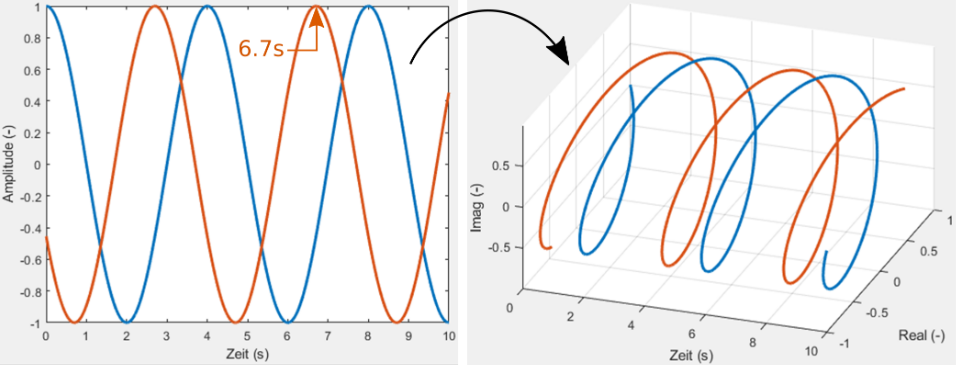
\includegraphics[width=0.5\textwidth]{papers/wavelets/images/10-3_PhaseShiftBsp.png}
	\caption{Grafische Wiedergabe der in den Matlabcode implementierten Phasenverschiebung, links Real und rechts komplexwertig.}
	\label{wavelet:fig:PhaseShiftBsp}
\end{figure}

\subsection{Amplitudenskalierung
	\label{wavelets:subsection:Amplitudenskalierung}}
In diesem Abschnitt geht es darum den Amplitudengang korrekt zu skalieren. Aus der vereinfachten Summenformel \[W_{a,b}=\sum_{a=f_0}^{a_n}\sum_{b=0}^{b_m}\frac{1}{N(a)}\sum_{n=0}^{N-1} x(n)\cdot\psi\left(\frac{t-b}{a}\right)\] ist die Gewichtung über die Anzahl Abtastpunkte in Abhängigkeit von $a$ gegeben. Der Grund ist die Gewichtung, die bereits im Morlet Wavelet vollzogen wird, über die Gauss'sche Fensterung mit der Funktion \[f(t)=e^{-\frac{\left(\frac{t-b}{a}\right)^2}{2}}.\]
Numerisch kann das relativ einfach gelöst werden, denn man braucht einfach gesagt nur die Wertigkeit des Fensters (Gauss verteilt) aufzusummieren.
Zum Vergleich in der DFT wird jeder Abtastpunkt gleich gewichtet, nämlich zu $100\%$, was gerade dem Faktor 1 entspricht (Abbildung \ref{wavelet:fig:AmpSklal1u2}).

\begin{figure}
	\centering
	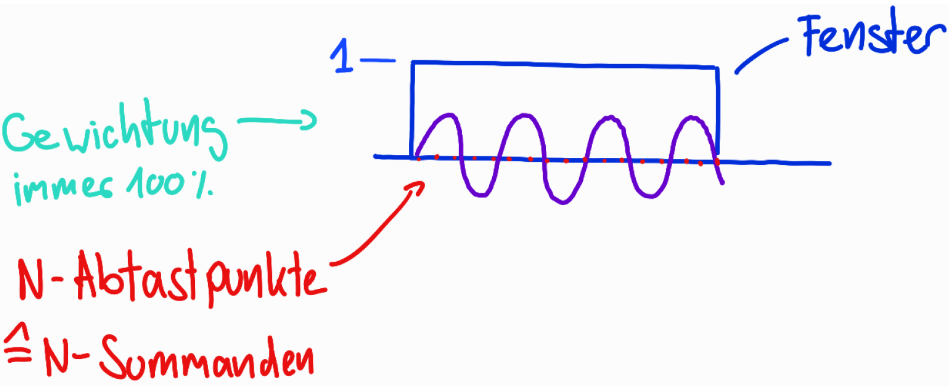
\includegraphics[width=0.35\textwidth]{papers/wavelets/images/11-1_AmpSklal1.png}
	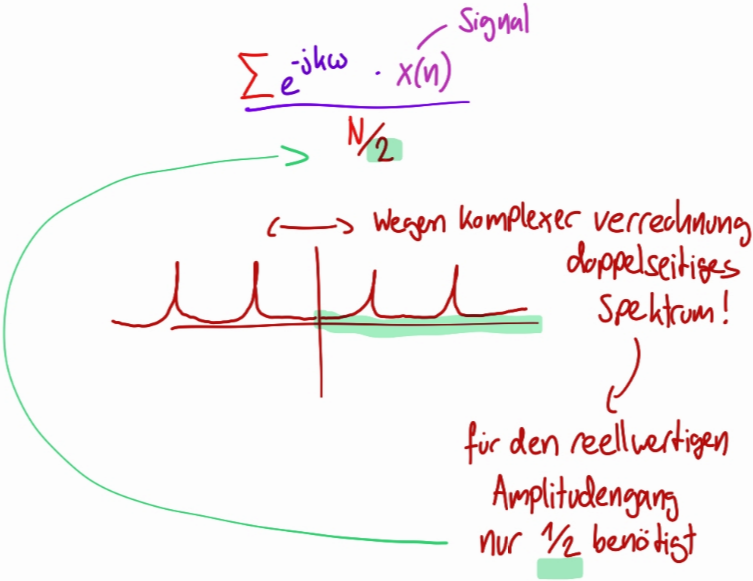
\includegraphics[width=0.35\textwidth]{papers/wavelets/images/11-2_AmpSklal2.png}
	\caption{Verfahren zur Mittelung der aufsummierten Werte in der DFT (analog in der FFT)}
	\label{wavelet:fig:AmpSklal1u2}
\end{figure}

Dadurch kann bei der DFT \[X(k)=\frac{\textbf{1}}{\textbf{N}}\sum_{n=0}^{N-1}x(n)\cdot e^{-j\frac{2\pi}{N}\cdot n}\] die Summe am Ende auch über die Anzahl Abtastpunkte geteilt werden (Abbildung \ref{wavelet:fig:AmpSklal3}).

\begin{figure}
	\centering
	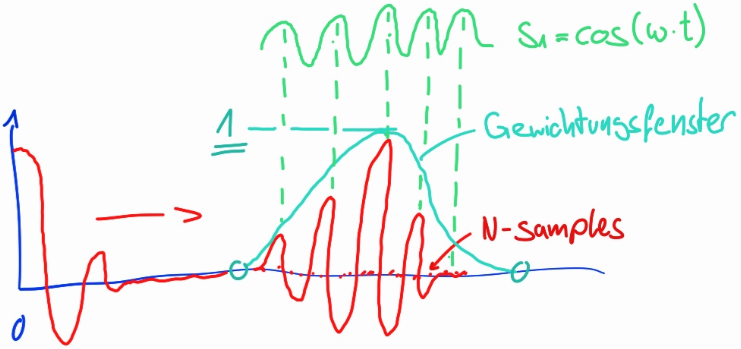
\includegraphics[width=0.35\textwidth]{papers/wavelets/images/11-3_AmpSklal3.png}
	\caption{Das Mittelungsverfahren bei der CWT grafisch interpretiert.}
	\label{wavelet:fig:AmpSklal3}
\end{figure}

Beim Wavelet muss jeder Abtastpunkt gemäss der Gaussverteilung gewichtet (Wert zwischen 0 – 1) und aufsummiert werden. Dadurch wird der Nenner in \[W_{a,b}=\sum_{a=f_0}^{a_n}\sum_{b=0}^{b_m}\frac{\textbf{1}}{\textbf{N(a)}}\sum_{n=0}^{N-1} x(n)\cdot\psi\left(\frac{t-b}{a}\right)\] eine Funktion von $N(a)$. D.h. die Gewichtung hängt direkt mit Dehnung oder Komprimierung der Grundfrequenz $f_0$ durch $a$ zusammen. Die Verschiebung $b$ nimmt keinen Einfluss, weil $b$ nur die Position auf der Zeitachse bestimmt, die Gewichtung bleibt aber pro Dehnungsfaktor $a$ von $f_0$ konstant.
Dabei muss man sich bewusst sein, durch die Verrechnung des Signals mit der komplexwertigen Funktion \[\psi(a,b)=Ke^{-j2\pi f_0\left(\frac{t-b}{a}\right)-\frac{\left(\frac{t-b}{a}\right)^2}{2}}\] bekommt man auch eine komplexwertige Funktion als Resultat. Dieses äussert sich als Spiegelung an der Ordinatenachse. Wird nun für den Amplitudengang nur der reellwertige Teil benötigt, muss auch nur durch die rechte Hälfte (kausale Seite) geteilt werden. Daher die Teilung durch $\frac{1}{N/2}$ bei der DFT und $\frac{1}{N(a)/2}$ bei der CWT (bezogen auf das Morlet Wavelet), zur Bestimmung des korrekten Amplitudenganges.

\subsection{Anwendung am einfachen Testsignal
	\label{wavelets:subsection:ErsteAnwendung}}
Das Testsignal wurde so festgelegt, dass die erwarteten Eigenschaften des CWT zur Geltung kommen können. Was ist damit gemeint? Die Fouriertransformation geht von unendlich langer Periodizität aus und funktioniert deshalb auch besonders gut für langanhaltende periodische Signale. In vielen realen Prozessen treten Effekte aber jeweils sehr kurzzeitig auf. Um den Umgang der Wavelettransformation mit kurzweiligen Signalen mit abrupten Änderungen besser zu verstehen sowie dem verhalten der FFT gegenüberzustellen, wurden kurzzeitig auftretenden Sinusschwingungen untersucht. Zu einem späteren Zeitpunkt wird das verhalten der CWT auch noch gegenüber einem verrauschten Signal untersucht(Abbildung \ref{wavelet:fig:ErsteAnwendung}).

\begin{figure}
	\centering
	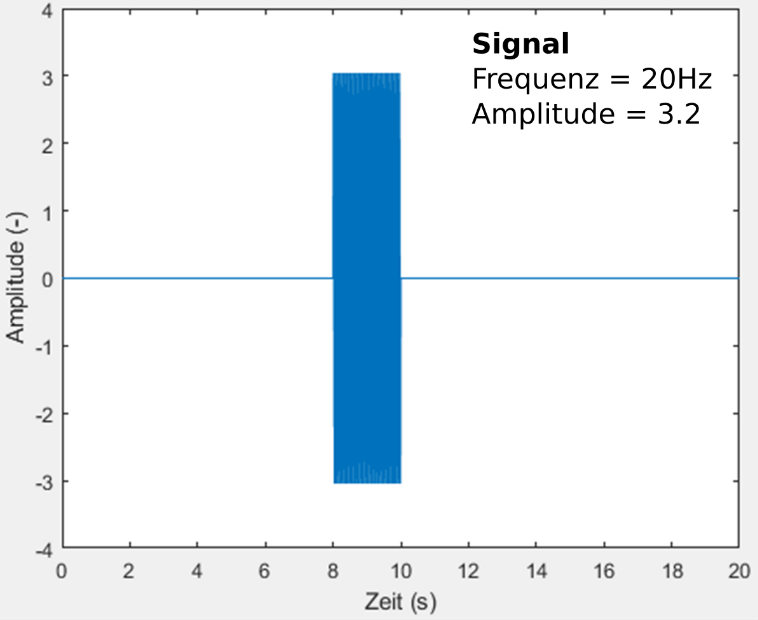
\includegraphics[width=0.2\textwidth]{papers/wavelets/images/8_BC_Signal.png}
	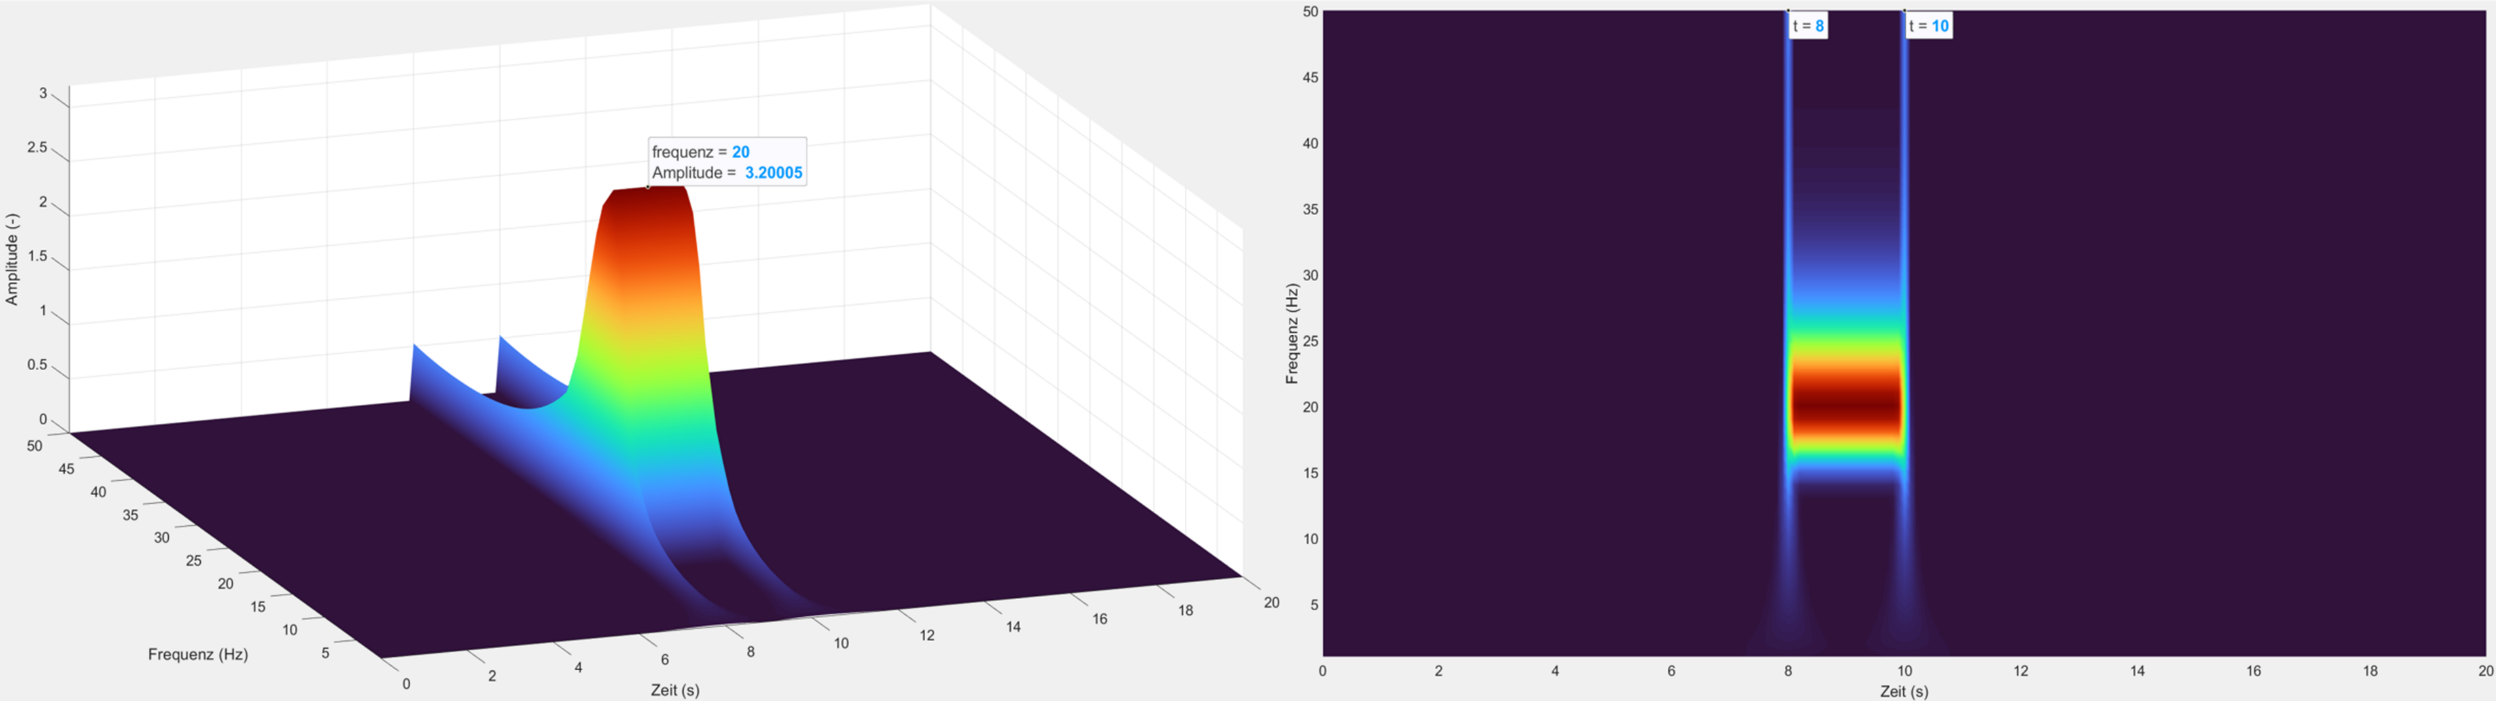
\includegraphics[width=\textwidth]{papers/wavelets/images/12-2_CWT-1Prog.png}
	\caption{Erste Anwendung des geschriebenen CWT-Code an einem einfachen Testsignal.}
	\label{wavelet:fig:ErsteAnwendung}
\end{figure}
